\newcommand{\namealine}{\textcolor{red}{Aline}}
\newcommand{\namebruno}{\textcolor{ForestGreen}{Bruno}}
\newcommand{\namecem}{\textcolor{blue}{Cem}}
\newcommand{\namedina}{\textcolor{orange}{Dina}}

\title[Daten Vorhersagen]{Daten Vorhersagen}
\date{\today}
\subtitle{Entscheidungsbäume}
\logo{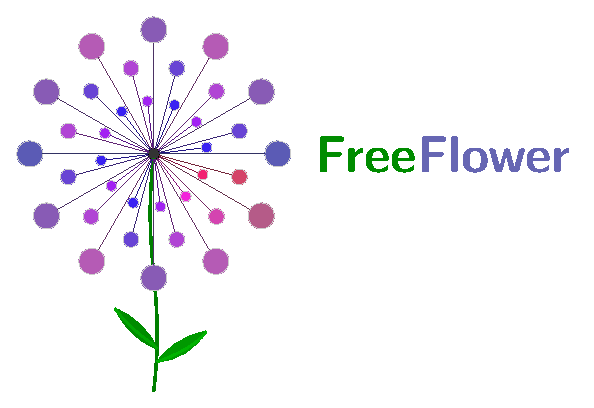
\includegraphics[width=.7cm]{Logos/FreeFlower.pdf}}

\frame{\titlepage}

\section{Entscheidungsbäume}

\begin{frame}{Themenübersicht}
    \begin{enumerate}
        \item[\faSquare] Grundidee
        \item[\faSquare] Gini-Koeffizient
        \item[\faSquare] Beispiel und Berechnung
        \item[\faSquare] Overfitting / Pruning
        \item[\faSquare] Bias und Feature Importance
        \item[\faSquare] Übungen und Notebook
    \end{enumerate}
\end{frame}

\begin{frame}{Grundidee}
    Ein Entscheidungsbaum teilt Daten schrittweise auf. Jede innere Knoten stellt eine Frage, jede Kante führt zu einer Teilmenge und jedes Blatt gibt die vorhergesagte Klasse an. Entscheidungsbäume sind gut interpretierbar und eignen sich für Klassifikationsaufgaben.
\end{frame}

\begin{frame}{Wie lernt ein Baum?}
    Der Baum wählt an jedem Knoten den Split, der die Daten am besten trennt. Ziel ist es, möglichst reine Blätter zu erzeugen. Typische Regularisierungen sind maximale Tiefe, minimale Blattgrösse oder minimale Impurity-Reduktion.
\end{frame}

\begin{frame}[fragile]{Gini-Koeffizient}
    \begin{tcolorbox}[colback=blue!5!white, colframe=blue!75!black, boxrule=0.8pt, enhanced, left=2mm, right=2mm, top=1mm, bottom=1mm, box align=base, title=Andrej A. Markov]
        \begin{minipage}{0.25\textwidth}
            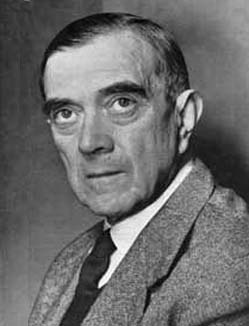
\includegraphics[width=\linewidth]{Grundlagen_Info/10_KI_und_Algorithmen/Figures/Corrado_Gini.jpg}
        \end{minipage}
        \hfill
        \begin{minipage}{0.7\textwidth}
            \begin{itemize}[<+->]
                \item Benannt nach Corrado Gini, einem italienischen Statistiker.
                \item Misst die Unreinheit eines Knotens: 0 = alle Beispiele gehören zur selben Klasse (reiner Knoten), 1 = gleichverteilt über alle Klassen.
                \item Bei der Auswahl eines Splits wird die gewichtete Gini-Reduktion berechnet, um den besten Split zu bestimmen.
            \end{itemize}
        \end{minipage}
    \end{tcolorbox}
    \[ \mathrm{Gini}(t) = 1 - \sum_{k=1}^K p_k^2\]
    Dabei ist $p_k$ der Anteil der Klasse $k$ im Knoten $t$.
\end{frame}

\begin{frame}{Beispiel: Auto-Besitz}
    \begin{center}
        \begin{table}[H]
            \centering
            \begin{tabular}{lcc|c}
                \toprule
                Person     & Einkommen & Alter & Auto \\
                \midrule
                \namealine & 35k       & 21    & Nein \\
                \namebruno & 60k       & 26    & Ja   \\
                \namecem   & 45k       & 28    & Nein \\
                \namedina  & 30k       & 40    & Ja   \\
                \bottomrule
            \end{tabular}
        \end{table}
    \end{center}
    
    Features \texttt{Einkommen} und \texttt{Alter}. Erste Aufteilung z. B. \texttt{Einkommen $>$ 50k?} führt zu Knoten mit unterschiedlichen Gini-Werten. (Beispiel detailliert im Skript.)
\end{frame}

\begin{frame}{Beispiel: Gini von Hand berechnen}
    Gegeben: 10 Personen, Marken A:4, B:3, C:2, D:1.
    \[   \mathrm{Gini} = 1 - (0.4^2 + 0.3^2 + 0.2^2 + 0.1^2) = 0.70    \]
\end{frame}

\begin{frame}[fragile]{Erstellung eines Baums (Übung)}
    Vorgehen: Wählen Sie mögliche Splits (z. B. \texttt{Lernzeit $>$ 5h?}, \texttt{Anwesenheit $>$ 80\%?}), berechnen Sie die Gini-Werte für Kinderknoten und wählen Sie den besten Split. Detaillierte Lösung im Skript.
\end{frame}

\begin{frame}{Overfitting und Underfitting}
    Ein unbeschränkter Baum kann Trainingsdaten auswendig lernen (Overfitting). Zu flache Bäume modellieren zu wenig Komplexität (Underfitting). Typische Gegenmassnahmen: Maximaltiefe, minimale Blattgrösse, Pruning.
\end{frame}

\begin{frame}{Pruning}
    Pruning reduziert die Komplexität nach dem Training, indem unwichtige Knoten entfernt oder zusammengeführt werden. Kriterien: minimale Anzahl Beispiele pro Blatt, minimale Verbesserung der Impurity.
\end{frame}

\begin{frame}{Bias in Entscheidungsbäumen}
    Obwohl Bäume interpretierbar sind, können sie historische Verzerrungen reproduzieren (z. B. Geografie im Credit Scoring). Achten Sie auf fehlende Kontextvariablen und prüfen Sie Fairness-Metriken.
\end{frame}

\begin{frame}{Feature Importance}
    Wichtigkeit eines Merkmals = Summe der Gini-Reduktionen über alle Splits auf diesem Feature. Bei einem einzelnen Baum ist die Wichtigkeit jedoch instabil; Random Forests liefern stabilere Schätzungen.
\end{frame}

\begin{frame}{Übungen und Notebook}
    Für praktische Übungen siehe das Jupyter-Notebook: %10_KI_und_Algorithmen/01_Entscheidungsbaum.ipynb. Bitte alle Code-Zellen ausführen und die Gini-Berechnungen nachrechnen.
\end{frame}

